\section{Supervisé : Lichess puis grands maîtres}

\subsection{Prétraining Lichess}

Le jeu de données vient du dump Lichess \code{standard rated} de février 2026,
filtré sur les deux joueurs à 1\,800 Elo ou plus
(\chemin{extract\_pgn\_from\_lichess.py}). Le fichier conservé,
\chemin{top\_games\_quality.pgn}, pèse 2,37 Go et contient exactement
1\,000\,000 de parties. Il a été converti en shards binaires
(\chemin{convert\_pgn\_to\_binary.py}) : des fichiers \code{.npz} de 500
parties, environ 16\,600 positions chacun, avec le tenseur
$119 \times 8 \times 8$ en \code{uint8}, l'indice de policy et le résultat.

Le dernier shard conservé porte l'indice 2399, ce qui indique environ
2\,400 shards, soit environ 1,2 million de parties et 39,9 M de positions.
Le fichier PGN conservé (1 M de parties) est donc légèrement plus petit que
l'entrée de conversion ; ce point est discuté en section~5.

L'entraînement utilise des shards mélangés (\chemin{sharded\_dataset.py}),
un lot de 4\,096, Adam à $10^{-3}$ et la précision mixte 16 bits. Le run
retenu a tourné 2 h 52 et s'est arrêté au bout de deux époques complètes,
19\,495 steps, soit 79,8 M d'échantillons vus.

\begin{figure}[h]
\centering
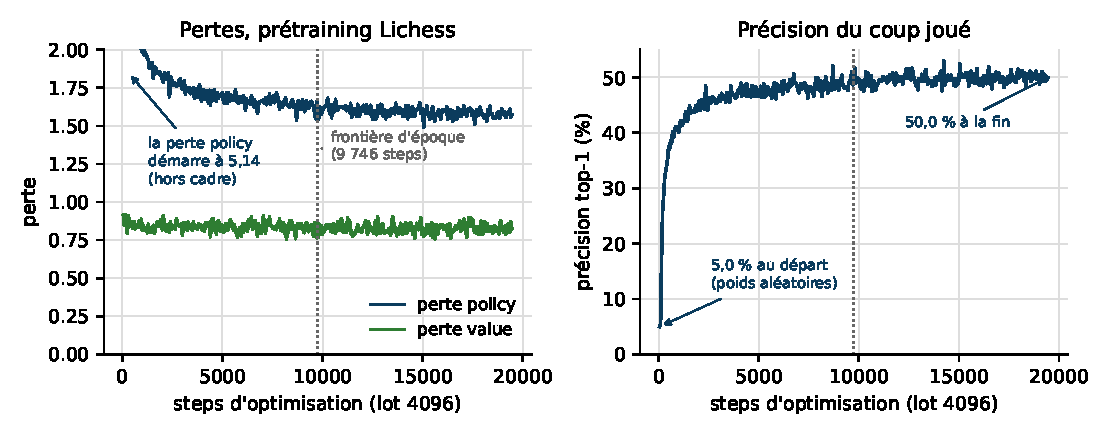
\includegraphics[width=\textwidth]{figures/fig_supervise_lichess.pdf}
\caption{Prétraining Lichess, run \code{jhqhhx5q}. À gauche, les pertes
policy et value sur une échelle linéaire plafonnée à 2, pour comparer
directement avec la figure~\ref{fig:gm} ; la perte policy démarre à 5,14,
au-dessus du cadre. La ligne pointillée marque la frontière d'époque à
9\,746 steps. À droite, la précision top-1 du coup joué, de 5,0 \% au départ
(poids aléatoires) à 50,0 \% à la fin.}
\label{fig:lichess}
\end{figure}

Les courbes de la figure~\ref{fig:lichess} sont le meilleur certificat de la
reprise de zéro : la précision démarre à 5 \%, la valeur typique d'un réseau
non entraîné, et non à 30 ou 40 \% comme pour un modèle déjà joueur. La perte
policy chute de 5,14 à 1,57, la perte value de 0,91 à 0,82. La petite marche
visible sur la perte policy au voisinage de la ligne pointillée correspond au
changement d'époque ; elle est bénigne et vient du brassage des shards.

\subsection{Affinage sur les parties de grands maîtres}

La deuxième phase reprend le checkpoint Lichess et l'affine sur les parties de
grands maîtres téléchargées depuis pgnmentor
(\chemin{download\_pgns.py}), nettoyées et dédoublonnées en un fichier par
partie (\chemin{clean\_pgns.7z}). Le script
(\chemin{train\_supervised.py}) change aussi de format : il lit directement
les PGN, sans passer par les shards, avec un lot de 2\,048.

Le jeu conservé dans \chemin{docs/clean\_pgns.7z} ne contient que 56\,562
parties, mais il s'agit d'un instantané partiel de mars. La taille réelle de
l'époque d'affinage se lit dans le checkpoint : 9\,498 lots de 2\,048, soit
19,45 M de positions par époque. Avec une moyenne de 91,5 plies par partie
(mesurée sur l'archive), cela représente environ 210\,000 parties.

Le run a duré 1 h 33 et fait exactement deux époques, 18\,996 steps, soit
38,9 M d'échantillons vus. Il s'arrête à l'époque 3 du compteur Lightning,
qui avait été hérité du checkpoint Lichess.

\begin{figure}[h]
\centering
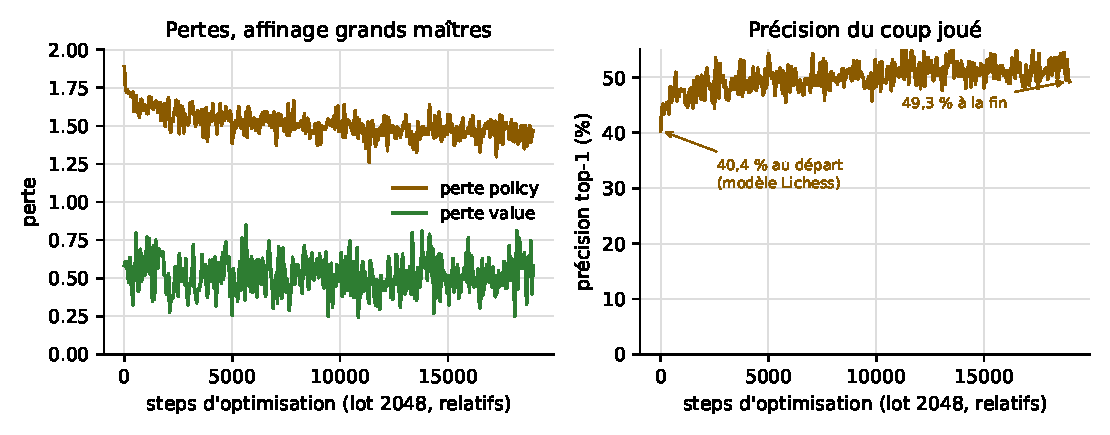
\includegraphics[width=\textwidth]{figures/fig_supervise_gm.pdf}
\caption{Affinage sur les grands maîtres, run \code{ifvh81l0}. Les steps sont
relatifs au début de l'affinage. La précision passe de 40,4 \% (modèle
Lichess) à 49,3 \%. La perte value reste plate autour de 0,58.}
\label{fig:gm}
\end{figure}

La figure~\ref{fig:gm} montre un régime différent du prétraining : à
l'échelle de ces deux époques, la perte policy baisse (1,89 à 1,47) et la
précision progresse de 40,4 \% à 49,3 \%, tandis que la perte value ne bouge
pratiquement pas (0,58). Autrement dit, l'affinage sert surtout à ajuster la
politique sur un style de jeu plus propre et plus tactique, pas à recalibrer
la valeur.

\subsection{Le transfert de poids testé puis abandonné}

Le soir du 6 avril, trois lancements du prétraining Lichess se succèdent. Les
deux premiers utilisent les poids transférés depuis l'ancien modèle ; le
troisième part de zéro. La figure~\ref{fig:transfert} compare les trois.

\begin{figure}[h]
\centering
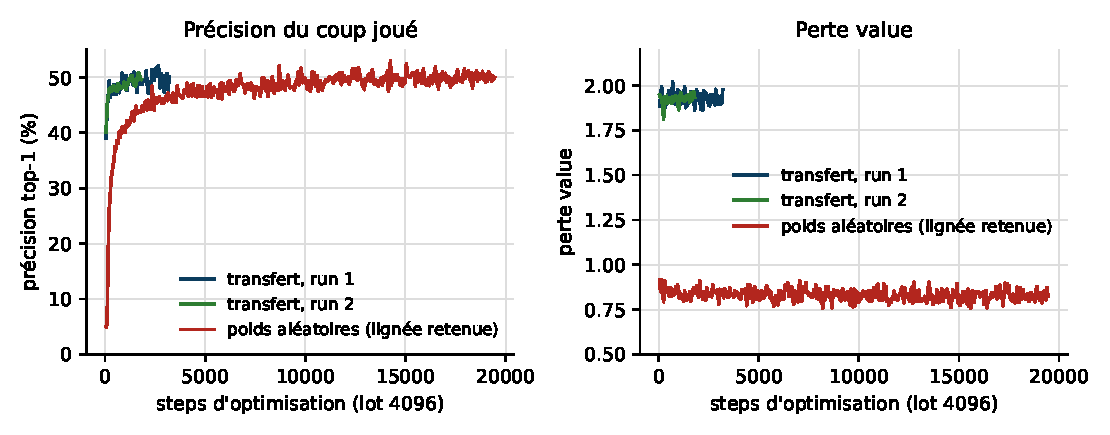
\includegraphics[width=\textwidth]{figures/fig_transfert.pdf}
\caption{Les trois lancements du prétraining Lichess du 6 avril. À gauche, la
précision top-1 : elle démarre à 39 et 40 \% pour les runs avec transfert, à
5 \% pour le run reparti de zéro. À droite, la perte value : elle reste
bloquée autour de 1,9 pour les runs transférés, contre 0,8 pour le run
retenu.}
\label{fig:transfert}
\end{figure}

Les deux runs transférés ont une précision de départ élevée (39 et 40 \%), ce
qui confirme que le transfert fonctionne pour l'essentiel du réseau. Mais leur
perte value reste autour de 1,9 pendant tout le run, deux fois pire qu'un
réseau aléatoire, alors que le run reparti de zéro la fait descendre sous
0,85. La tête de value transférée est donc inadaptée à la nouvelle
architecture, ou à la convention de signe du jeu de données. Les deux runs
ont été interrompus après 3\,200 et 1\,800 steps ; le troisième, sans
transfert, a été mené au bout.

\begin{attention}
La lignée du modèle actuel ne contient pas les poids transférés. Les fichiers
\code{modele\_generation0\_init.pt} et
\code{alphazero-supervised-step=3000.ckpt}, dans le dossier
\chemin{python\_src/checkpoints}, conservent la trace de cet essai, mais ils ne
font pas partie de l'ascendance de l'iter436. Le modèle est bien reparti de
zéro au stade supervisé.
\end{attention}
